\documentclass{article}
\usepackage{graphicx}
\usepackage{amsmath}
\usepackage{amsfonts}
\renewcommand{\baselinestretch}{1}
\setlength{\textheight}{9in}
\setlength{\textwidth}{6.5in}
\setlength{\headheight}{0in}
\setlength{\headsep}{0in}
\setlength{\topmargin}{0in}
\setlength{\oddsidemargin}{0in}
\setlength{\evensidemargin}{0in}
\setlength{\parindent}{.3in}
\graphicspath{{images/}}

\title{Communication Systems \\
    \large Chapter 3 Analysis and Transmission of Signals}
\author{Hunter Mills}
\date{\today}

\begin{document}
    \maketitle

    \medskip
    
    \section{Fourier Transform of Signals}
    The \textbf{Fourier Transform} of $g(t)$ is defined as
    \begin{equation}
        G(f) = \mathfrak{F} [g(t)] = \int_{-\infty}^{\infty}g(t)e^{-j2\pi ft}dt
    \end{equation}
    The \textbf{Inverse Fourier Transform} is defined as
    \begin{equation}
        g(t) = \mathfrak{F}^{-1} [G(f)] = \int_{-\infty}^{\infty}G(f)e^{j2\pi ft}dt
    \end{equation}

    \subsection{Conjugate Symmetry Property}
    If $g(t)$ is real then $G(f)$ and $G(-f)$ are complex conjugates, that is
    \begin{equation}
        G(-f) = G^*(f) = \int_{-\infty}^{\infty}g(t)e^{j2\pi ft}dt
    \end{equation}
    \begin{equation}
        |G(-f)| = |G(f)|
    \end{equation}
    \begin{equation}
        \theta_g(-f) = -\theta_g(f)
    \end{equation}
    For real signals $g(t)$ the amplitude spectrum is even and the phase spectrum is odd. 

    \subsection{Existence of the Fourier Transform}
    If a signal satisfies the following condition then the signal has a fourier transform.
    \begin{equation}
        \int_{-\infty}^{\infty}|g(t)|dt < 0
    \end{equation}

    There is a Fourier Transform table on page 106 of the textbook.

    \section{Some Fourier Transform Properties}
    I will only note specific properties, the others are in a table on page 123 of the text book.

    \subsection{Time-Frequency Duality}
    The operations required to go from $g(t)$ to $G(t)$ and then from $G(t)$ to $g(t)$ are very similar, only differing in the signs of the exponential.
    This is the basis of the duality of time and frequency. For any relationship between $g(t)$ and $G(f)$ there exists a dual relationship obtained 
    by interchanging the roles of $g(t)$ and $G(f)$. For example the time-shifting property 
    \begin{equation}
        g(t-t_0) \leftrightarrow G(f)e^{-j2\pi ft_0}
    \end{equation}
    and the dual of this property 
    \begin{equation}
        g(t)e^{-j2\pi f_0t} \leftrightarrow G(f-f_0)
    \end{equation}

    \begin{figure}[h]
        \centering
        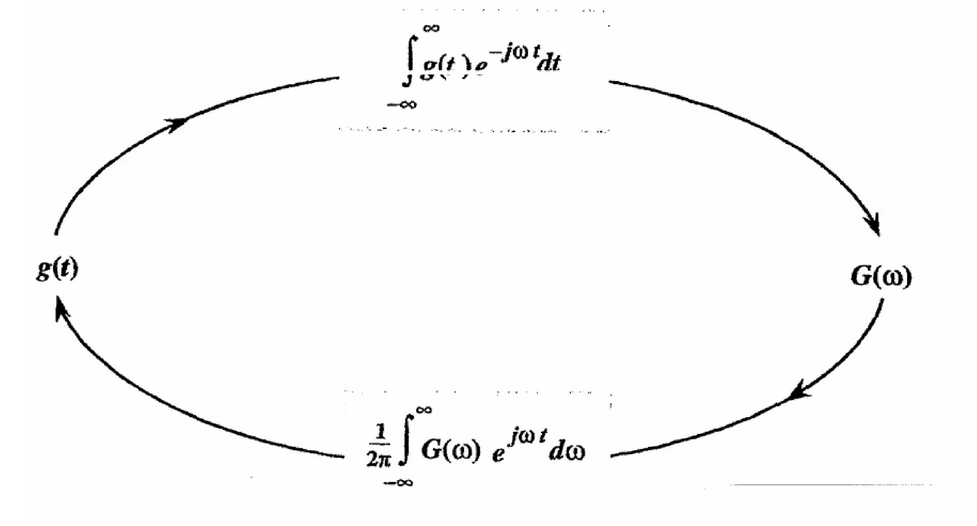
\includegraphics[width=0.75\textwidth]{td}
        \caption{Near symmetry between Fourier and Inverse Fourier Transforms}
    \end{figure}

    \subsection{Reciprocity of Signal Duration and its Bandwidth}
    The time-scaling property implies that if $g(t)$ gets wider (time extension) its spectrum gets narrower and the reverse, if $g(t)$ is time compressed 
    the spectrum gets wider. The bandwidth of a signal is inversely proportional to the signal duration.

    \subsection{Convolution}
    Convolution is defined as 
    \begin{equation}
        g(t) \ast w(t) = \int_{-\infty}^{\infty}g(\tau)w(t-\tau)d\tau
    \end{equation}

    \section{Signal Transmission Through a LTI System}
    The LTI system model shown in the next figure can be used to characterize communication channels. A stable LTI system can be characterized in 
    the time domain by its impulse response $h(t)$ which is the system response $y(t)$ to a unit impulse $x(t) = \delta(t)$.

    \begin{figure}[h]
        \centering
        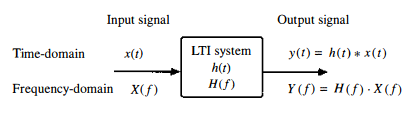
\includegraphics[width=0.75\textwidth]{lti}
        \caption{Signal Transmission through a LTI system}
    \end{figure}

    \begin{equation}
        y(t) = h(t) \ast x(t)
    \end{equation}
    and when $x(t) = \delta(t)$, $y(t) = h(t)$.
    \begin{equation}
        Y(f) = H(f)X(f)
    \end{equation}
    The fourier transform of the impulse response is referred to as the \textbf{transfer function} or the \textbf{frequency response}. In general $H(f)$ is 
    complex and can be written as 
    \begin{equation}
        H(f) = |H(f)|e^{j\theta_h(f)}
    \end{equation}

    \subsection{Signal Distortion During Transmission}
    \begin{equation}
        |Y(f)| = |X(f)||H(f)|
    \end{equation}
    \begin{equation}
        \theta_y(f) = \theta_x(f) + \theta_h(f)
    \end{equation}

    \subsection{Distortionless Transmission}
    It is of practical interest to determine the characteristics of a system that allow for \textbf{Distortionless Transmission}. In distortionless transmission
    satisfies the following
    \begin{equation}
        y(t) = kx(t-t_d)
    \end{equation}
    The transfer function (frequency response) required for distortionless transmission is
    \begin{equation}
        |H(f)| = k
    \end{equation}
    \begin{equation}
        \theta_h(f) = -2\pi ft_d
    \end{equation}
    That says the amplitude response must be a constant and the phase response must be linear and go through the origin. If the slope is not linear
    then components of different frequencies undergo different time delays. The \textbf{group delay, $t_g$,} is when the output envelope is the same as the input
    envelope delayed by $t_g$.
    \begin{equation}
        t_g = t_d(f) = -\frac{1}{2\pi}\frac{d\theta_h(f)}{df}
    \end{equation}

    \section{Ideal vs Practical Filters}
    Ideal filters allow distortionless transmission over a certain band while completely suppressing signals outside that band.

    \begin{figure}[h]
        \centering
        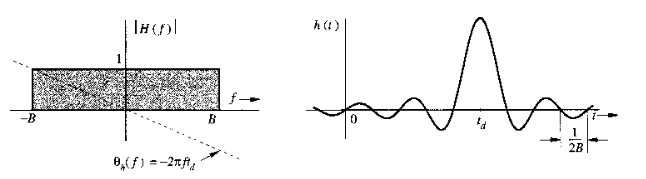
\includegraphics[width=0.75\textwidth]{lp}
        \caption{Ideal Low Pass Filter}
    \end{figure}

    \begin{figure}[h]
        \centering
        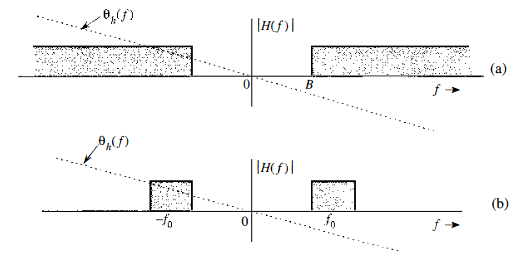
\includegraphics[width=0.75\textwidth]{hp_bp}
        \caption{Ideal High and Band Pass Filter}
    \end{figure}

    \subsection{Practically Realizable Filters}
    For physically realizable system $h(t)$ must be casual. This is equivalent to the Paley-Wiener criterion in the frequency domain that states that
    necessary and sufficient condition for $|H(f)|$ to be the amplitude response of a casual system:
    \begin{equation}
        \int_{-\infty}^{\infty}\frac{|ln|H(f)||}{1+(2\pi f)^2}df < \infty
    \end{equation}
    This states that $|H(f)|$ cannot be $0$ over a band. You can create a causal system by $\hat{h}(t) = h(t)u(t)$ and with sufficient time delay it
    will be close to the ideal filter. The trade off is the much higher delay in the output. The \textbf{cutoff frequency} of a filter is the 3db (half power)
    bandwidth.

    \section{Signal Energy and Energy Spectral Density}
    The energy $E_g$ of a signal $g(t)$ is defined as the area under $|g(t)|^2$.
    \subsection{Parseval's Theorem}
    \begin{equation}
        E_g = \int_{-\infty}^{\infty}|G(f)|^2df = \int_{-\infty}^{\infty}g^2(t)dt
    \end{equation}

    \subsection{Energy Spectral Density (ESD)}
    We can interpret $|G(f)|^2$ as the energy per unit bandwidth (in Hz) of $g(t)$. The \textbf{energy spectral density (ESD, $ \varPsi_g(f)$)} is defined
    as 
    \begin{equation}
        \varPsi_g(f) = |G(f)|^2
    \end{equation}
    and the energy from Parseval's Theorem can be defined as
    \begin{equation}
        E_g = \int_{-\infty}^{\infty}\varPsi_g(f)df
    \end{equation}

    \subsection{Time Autocorrelation Function and ESD}
    There is a very important relationship between the autocorrelation $\psi_g(\tau)$ 
    and its ESD $\varPsi_g(f)$. The autocorrelation function and its ESD form a Fourier Transform pair known as the \textbf{Wiener-Khintchine Theorem}.

    \begin{equation}
        \psi_g(\tau) \leftrightarrow \varPsi_g(f) = |G(f)|^2
    \end{equation}
    This is also valid for complex signals.

    \section{Signal Power and Power Spectral Density}
    The power of a real $g(t)$ is
    \begin{equation}
        P_g = \lim_{T \rightarrow \infty}\frac{1}{T}\int_{-T/2}^{T/2}g^2(t)dt
    \end{equation}
    The relationship between power and energy of non-periodic signals is 
    \begin{equation}
        P_g = \lim_{T \rightarrow \infty}\frac{E_{gT}}{T}
    \end{equation}
    where $E_{gT}$ is the energy of a truncated $g(t)$ over a period. 

    \subsection{Power Spectral Density (PSD)}
    The \textbf{Power Spectral Density} is defined as
    \begin{equation}
        S_g(f) = \lim_{T \rightarrow \infty} \frac{|G_T(f)|^2}{T}
    \end{equation}
    where $G_T(f)$ is the fourier transform of a truncated $g(t)$ over a period.
    \begin{equation}
        P_g = 2\int_{0}^{\infty}S_g(f)df
    \end{equation}

    \subsection{Time Autocorrelation Function of Power Signals}
    The time autocorrelation function $\mathfrak{R}_g(\tau)$ of a real power signal $g(t)$ is
    \begin{equation}
        \mathfrak{R}_g(\tau) = \lim_{T \rightarrow \infty} \frac{1}{T}\int_{-T/2}^{T/2}g(t)g(t-\tau)dt
    \end{equation}
    $\mathfrak{R}_g(\tau)$ is a even function of $t$ so
    \begin{equation}
        \mathfrak{R}_g(\tau) = \mathfrak{R}_g(-\tau)
    \end{equation}
    The Wiener-Khintchine theorem states
    \begin{equation}
        \mathfrak{R}_g(\tau) \leftrightarrow \lim_{T \rightarrow \infty} \frac{|G_T(f)|^2}{T} = S_g(f)
    \end{equation}

    \begin{figure}[h]
        \centering
        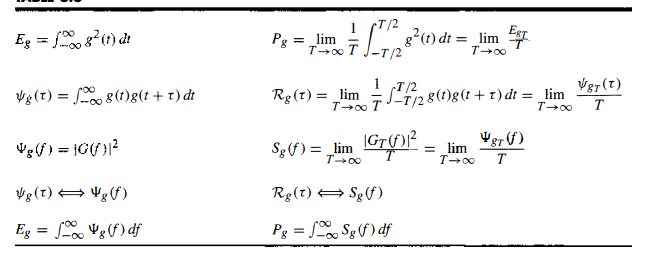
\includegraphics[width=0.75\textwidth]{e_v_p}
        \caption{Signal Energy vs Signal Power}
    \end{figure}

    \subsection{Signal Power is its Mean Square Value}
    Defining $< >$ as the time average
    \begin{equation}
        P_g = <g^2(t)> = \lim_{T \rightarrow \infty}\int_{-T/2}^{T/2}g^2(t)dt
    \end{equation}
    The RMS value is $[g(t)]_{RMS} = \sqrt{P_g}$

    \begin{equation}
        \mathfrak{R}_g(\tau) = <g(t)g(t\pm \tau)>
    \end{equation}

    \subsection{Input PSD vs Output PSD}
    \begin{equation}
        S_y(f) = |H(f)|^2S_g(f)
    \end{equation}

    \end{document}